\chapter{Appendix III}
\label{chap-app-imit}
\begin{figure}[b]
    %\vspace{-0.12cm}
    \centering
    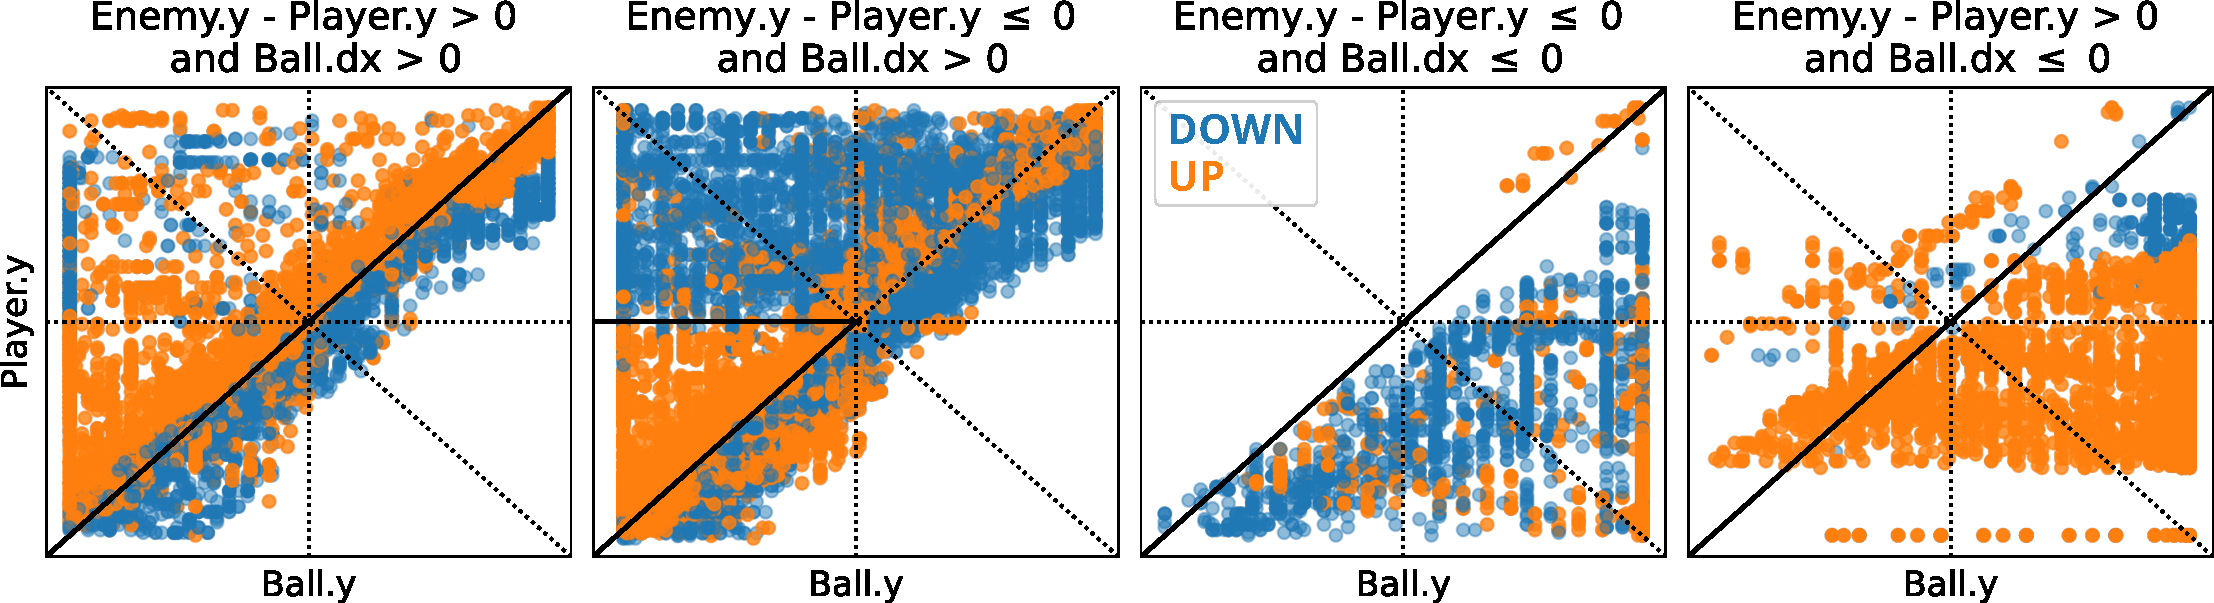
\includegraphics[width=1.\textwidth]{images/images_part3/pong_state_space.pdf}
    %\vspace{3mm}
    \caption{\textbf{Oracle decision rules are oblique} illustrated on PPO for different state space partitions of the Pong environment. Decisions boundaries are both oblique and parallel.}
    \label{fig:pong_states}
\end{figure}

\textbf{Oblique decision trees.} One can imitate oracles with programs that make tests of linear combinations of features. Many oracles learn oblique or more complex decision rules over an MDP state space. This is illustrated in Figure~\ref{fig:pong_states} where a PPO neural oracle creates oblique partitions of the state-space for the Pong environments. Programs that test only individual features would fail to fit this partition (\cf Figure~\ref{fig:pong_states}). 
We thus modify CART~\citep{breiman}, an algorithm returning an axes-parallel trees for regression and supervised classification problems, for it to return oblique decision trees. 
% Essentially, oblique trees trade-off interpretability of axes-parallel trees for better expressivity: each oblique tree node tests a linear combination of features. 
In addition to single feature tests, our oblique trees consider linear combinations of two features with weights $1$ and $-1$, \eg\@ for MDP states $s_i \in \mathbb{R}^{p}$, the oblique features values are $s^{oblique}_i = \{s_{i1} - s_{i0}, s_{i2} - s_{i0}, ..., s_{ip} - s_{i0}, ...,s_{ip-1} - s_{ip}\} \in \mathbb{R}^{p^2}$. For example, using an oracle dataset with $n$ state-actions pairs: $(\bar{S}, \Bar{A} = \pi^{*}(\bar{S})) \subsetneq \mathbb{R}^{n\cdot(p+\dim(A))}$, we obtain oblique decision trees by fitting $(\bar{S},\bar{S}^{oblique} , \Bar{A} = \pi^{*}(\bar{S})) \subsetneq \mathbb{R}^{n\cdot(p(p+1)+\dim(A))}$. 
Given $\bar{S}$, computing $\bar{S}^{oblique}$ can be done efficiently by computing the values of the lower (or upper) triangles in the $\bar{S} \otimes \bar{S} - (\bar{S} \otimes \bar{S})^T$ tensor (excluding the diagonals) (\cf line~\ref{alg:oblique2} of Algorithm~\ref{alg:iqdagger}). We further demonstrate the superiority of oblique trees in our experimental evaluation on a diverse set of RL tasks.


\section{All interpretability-performance trade-offs}
In this appendix we provide the interpretability-performance trade-offs of all the tested environments. All the measures come from the experiment from Section \ref{sec:res-trade-offs}.

\begin{figure}
    \centering
    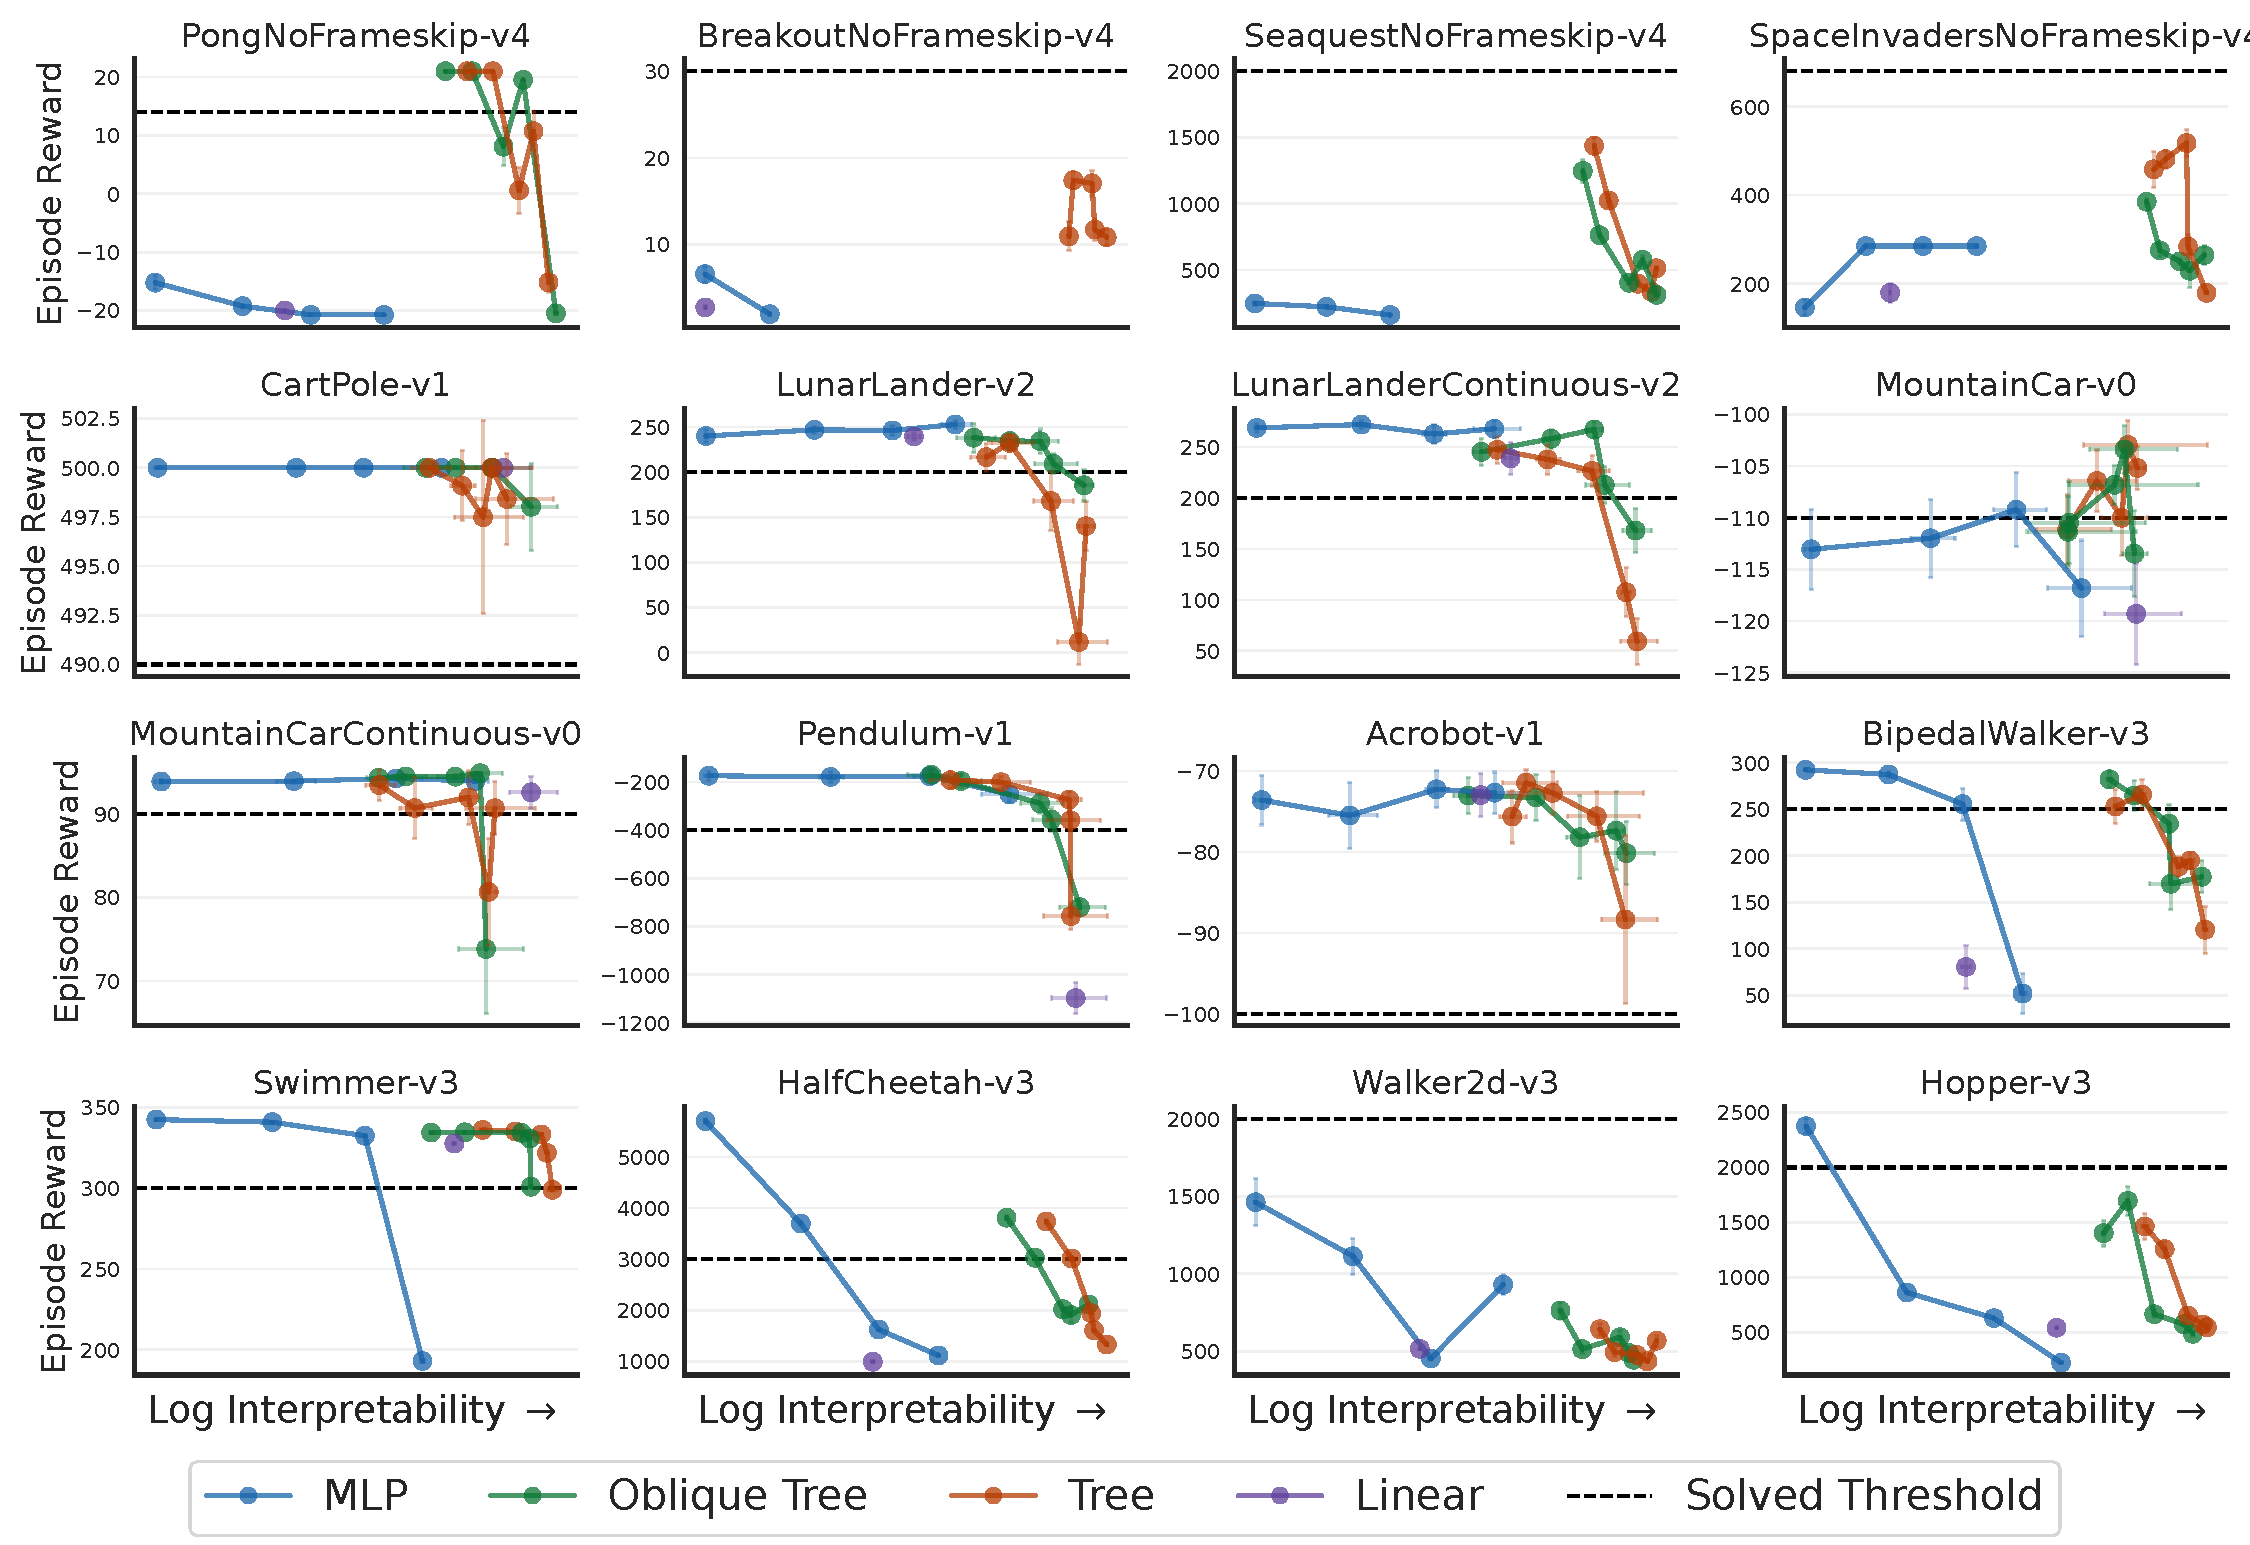
\includegraphics[width=1\linewidth]{images/images_part3/trade_off_step_times.pdf}
    \caption{Trade-off Cumulative Reward vs. Step Inference Time}
    \label{fig:trade-off}
\end{figure}

\begin{figure}[ht]
    \centering
    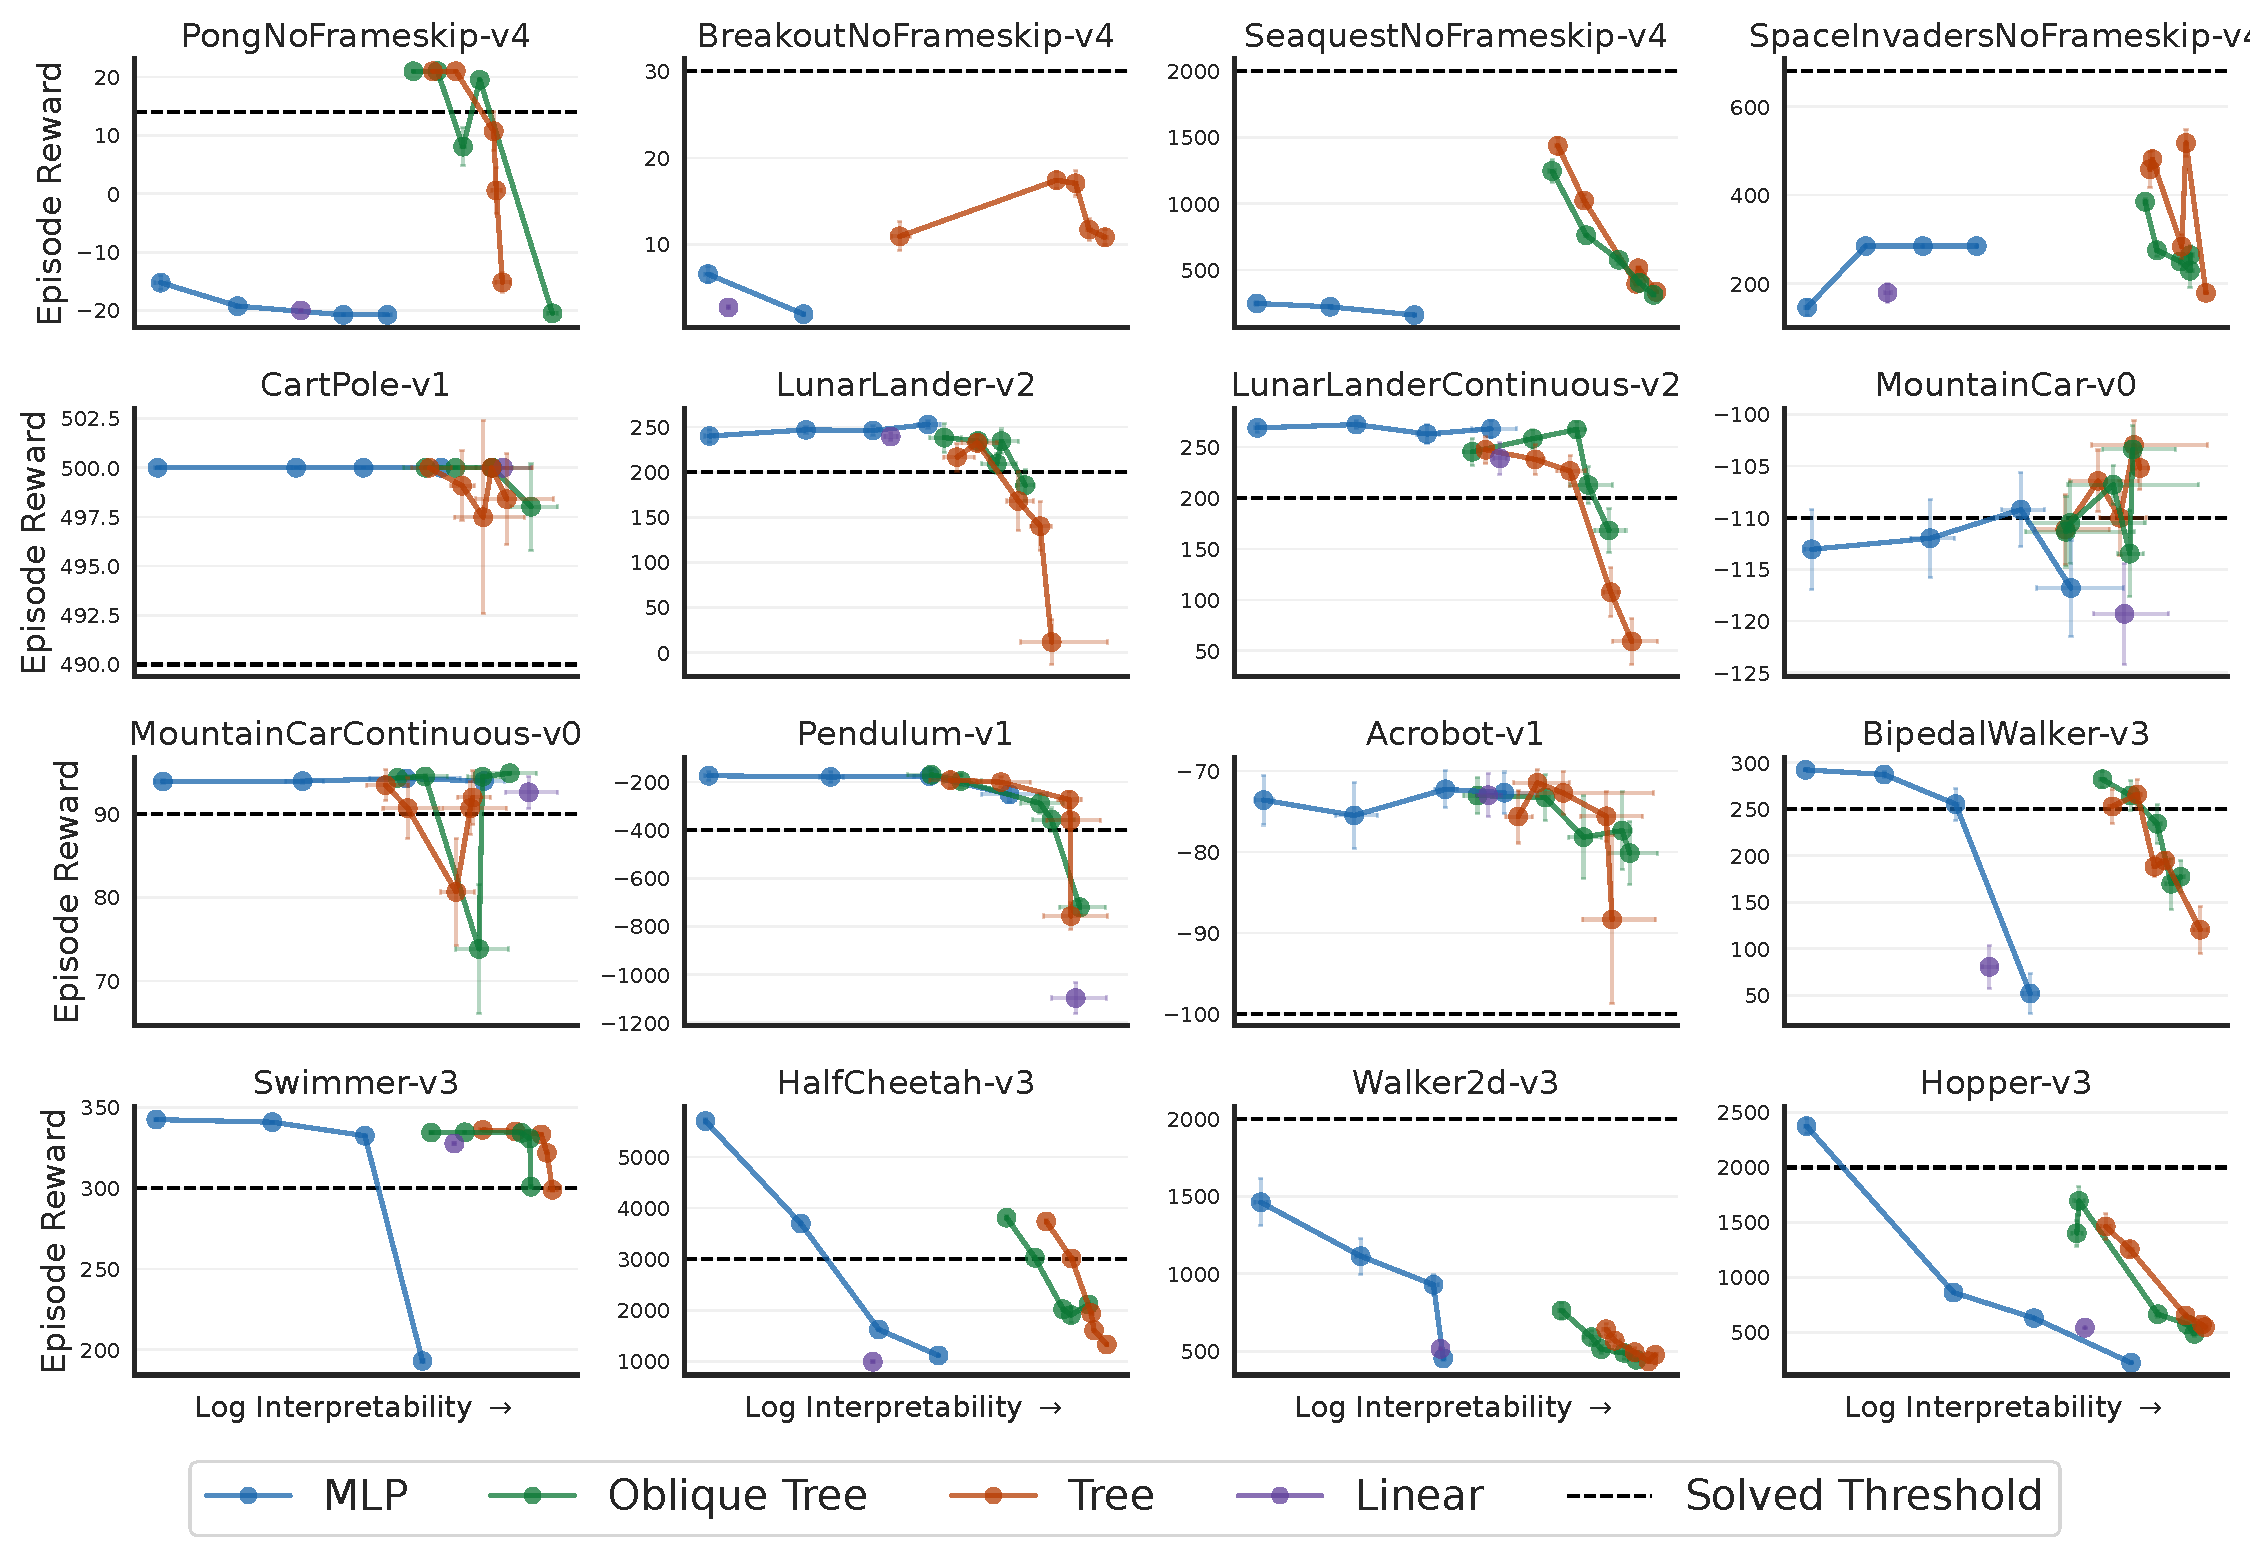
\includegraphics[width=0.95\linewidth]{images/images_part3/trade_off.pdf}
    \caption{Trade-off Cumulative Reward vs. Episode Inference Time}
    \label{fig:trade-off-episode}
\end{figure}

\begin{figure}[ht]
    \centering
    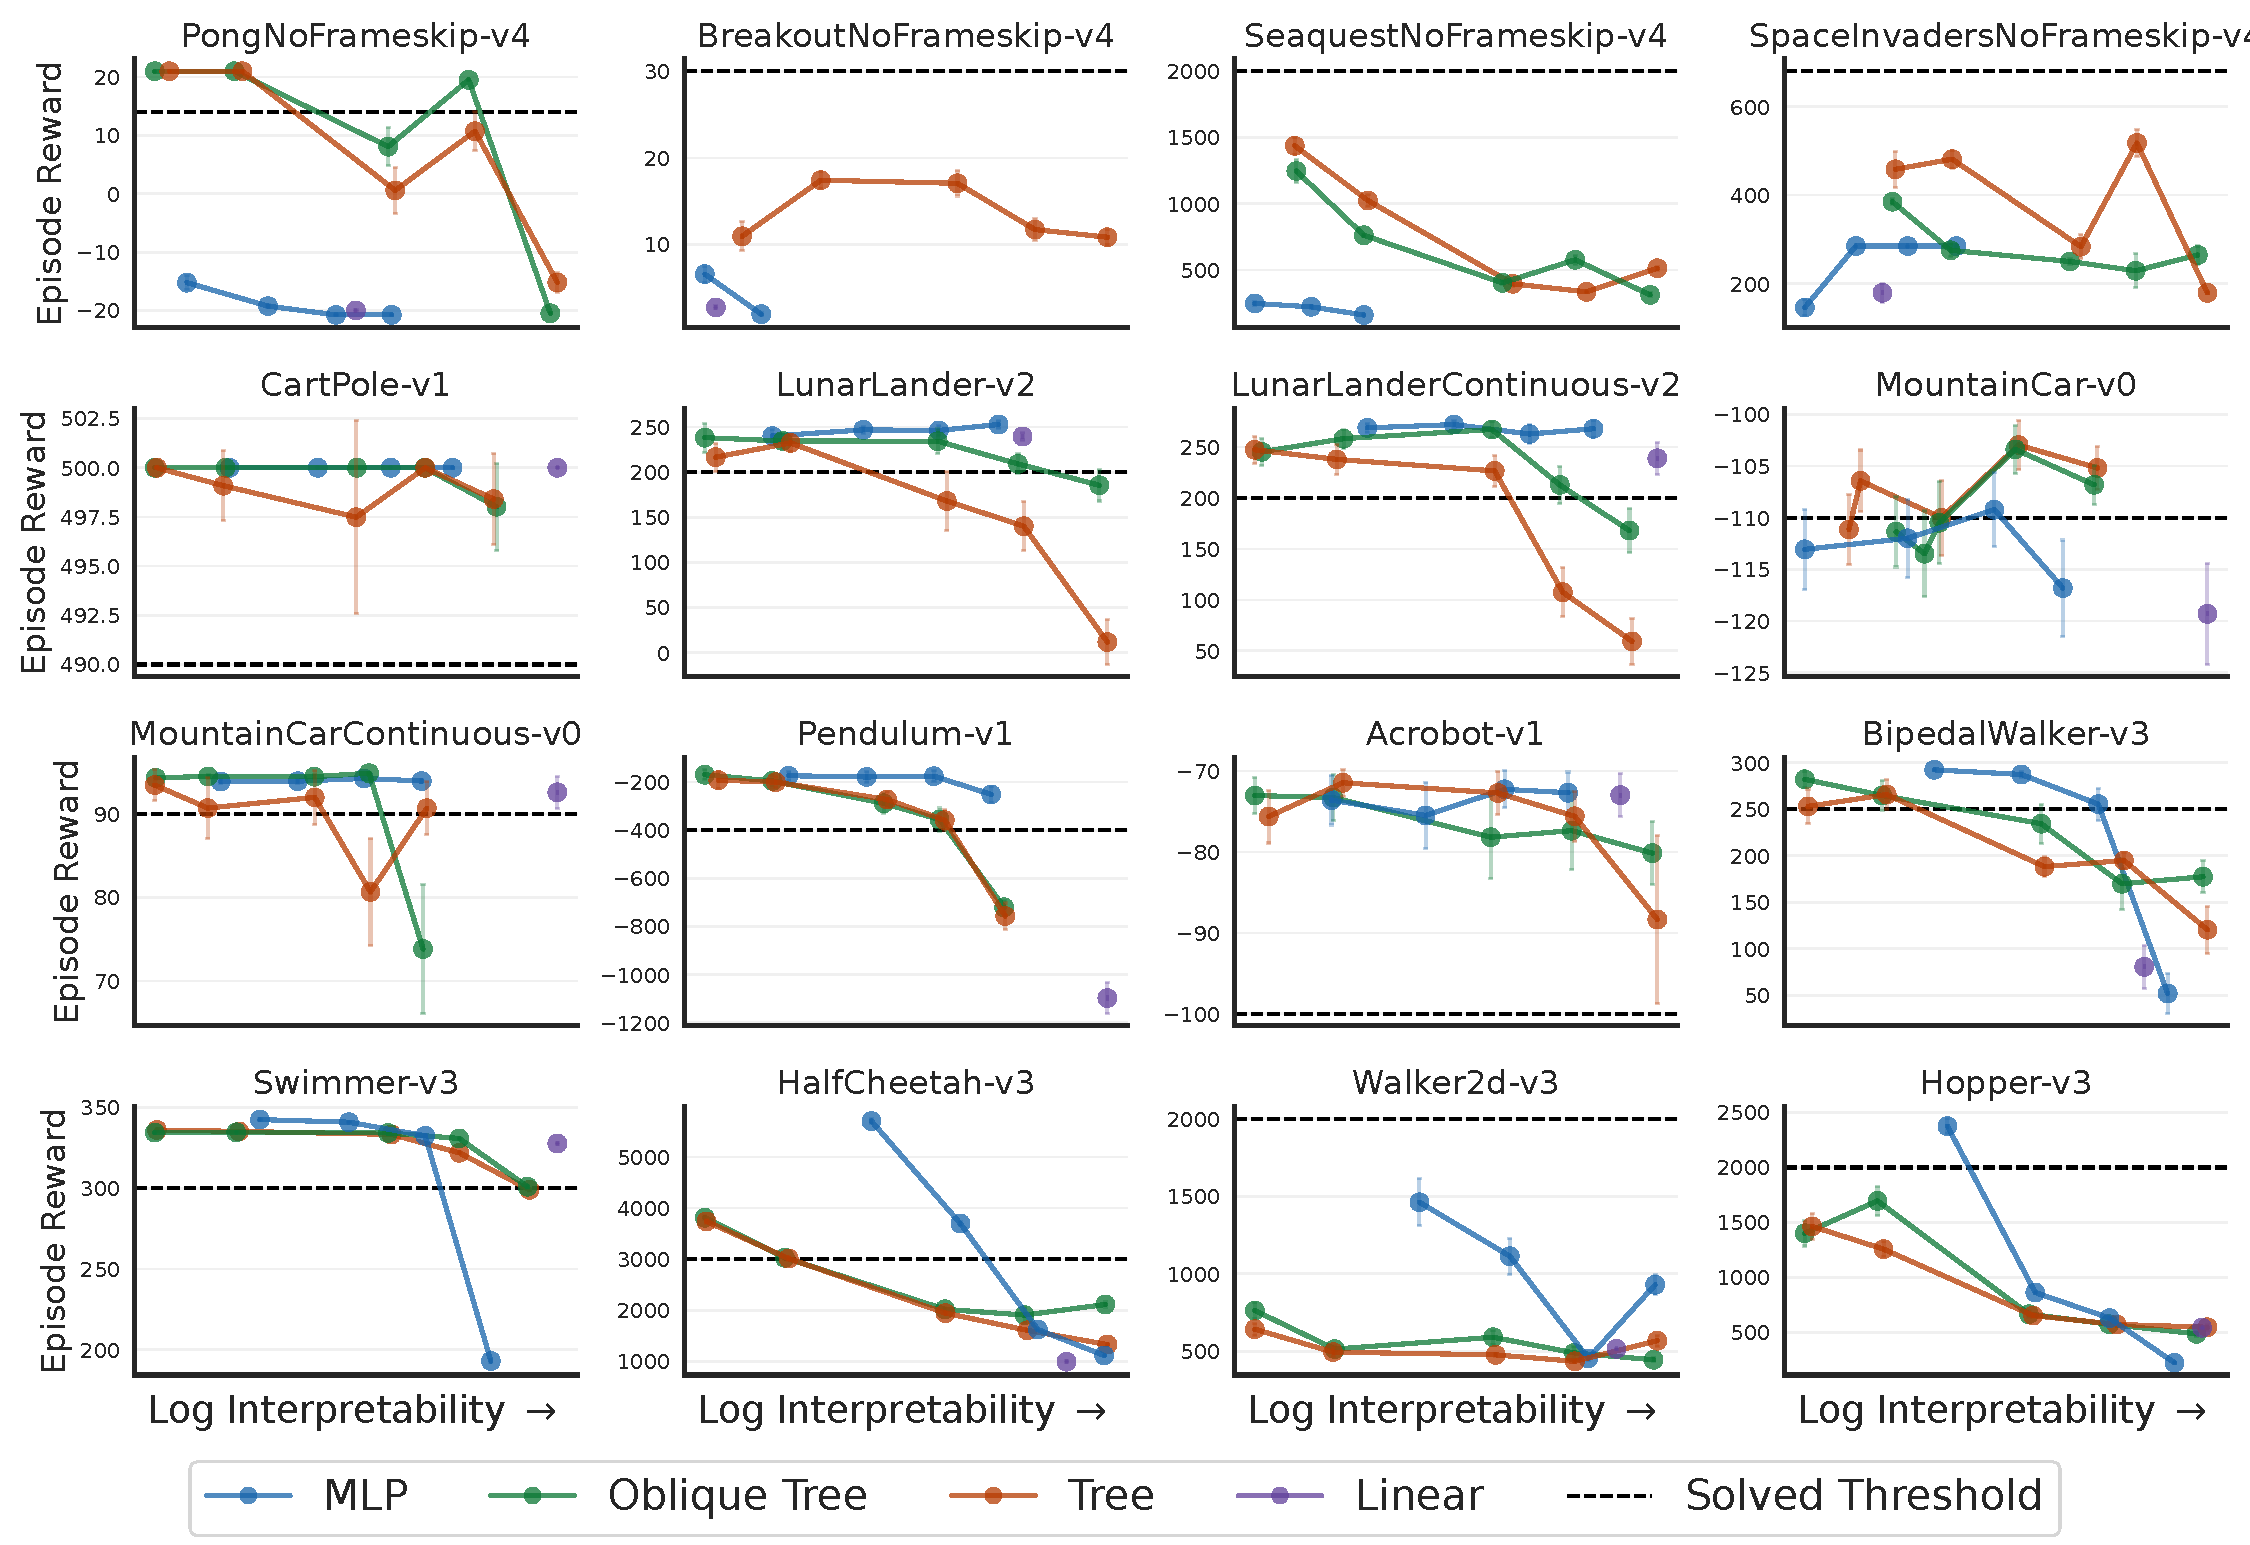
\includegraphics[width=0.95\linewidth]{images/images_part3/trade_off_size.pdf}
    \caption{Trade-off Cumulative Reward vs. Policy Size}
    \label{fig:trade-off-size}
\end{figure}